
\documentclass[../GE_Recitation.tex]{subfiles}

\begin{frame}{L\'{e}on Walras (1834--1910)\dots}
\begin{figure}
	\centering
	\includegraphics[width=0.5\linewidth]{walras_pic}
	\label{fig:walraspic}
\end{figure}
\end{frame}

\begin{frame}{\dots and his life}
	\begin{itemize}
		\item Born in \'{E}vreux, France in 1834;
		\item Failed college admission twice, studies to become an engineer but\dots
		\item \dots spends time writing two failed novels, that he has to publish with his own money because nobody wants them;
		\item In 1858, his father persuades him to work on Econ, so he finally drops out of college;
		\item 1860: He goes to Switzerland to try to advocate full land collectivization, but he fails, so he decides to start a cooperative bank with some friends (among which the grandson of famous French economist Jean-Baptiste Say);
		\item 1869: his bank fails.
		\item 1871: He applies to become a professor in Lausanne, arguing that economics has to become more mathematical;
		\item 1872: publishes his treaty ``Elements of Pure Political Economy''. Published in 100 copies thanks to the benevolence of some friend in the government.
		\item 1906: He applies (??!!) to the Nobel Peace prize because he is broke. Too bad Teddy Roosevelt was in the contest that year.
	\end{itemize}
\end{frame}


\begin{frame}{General Equilibrium in Pure Exchange}
A General Equilibrium is a set of \textbf{prices} $\left\lbrace p_1, p_2\right\rbrace$, and \textbf{allocations} for consumption  $\left\lbrace \underline{c}_1, \underline{c}_2\right\rbrace$ such that, given initial endowments of goods $\underline{e}_1, \underline{e}_2$:
\begin{enumerate}
	\item Consumers choose consumption $\left\lbrace \underline{c}_1, \underline{c}_2\right\rbrace$ subject to their budget constraint for given \textbf{prices};
	\item  The good markets clear.
\end{enumerate}
\end{frame}



\begin{frame}{Solving GE}
		\begin{enumerate}
			\item Technology $\Rightarrow$ PPF;
			\item Preferences $\Rightarrow$ Indifference curves;
			\item  Endowments with 1 and 2 $\Rightarrow$ price ratio.
		\end{enumerate}
\end{frame}

\begin{frame}{Solving GE in Pure Exchange}
GE is given by the point \textbf{in the Edgeworth box} such that indifference curves are tangent to each other and utility is maximized for given initial endowments, and the price ratio that is tangent to the indifference curves.\\
Steps:
\begin{enumerate}
	\item Solve the consumer problem for given income $I$ for both consumers;
	\item For each consumer, set $I = p_1e_1 + p_2e_2$, find $c_1, c_2$ as a function of price ratio;
	\item Impose market clearing: $c^1_1 + c^2_1 = e^1_1 + e^2_1 = E_1$.\footnote{Superscripts denote the agent's identity, subscripts the goods.}
\end{enumerate}
\end{frame}

\begin{frame}{Edgeworth Box: An example}
Consider an economy with two goods, x and y, and two agents, A and B, with preferences:
\begin{equation}\label{Ua}
U^A(x^A, y^A) = x^A\times y^A,
\end{equation}
\begin{equation}\label{Ub}
U^B(x^B, y^B) = (x^B)^\frac{2}{3}\times(y^B)^\frac{1}{3},
\end{equation}
denote the price ratio $p_y/p_x \equiv p$ (level does not matter), and let the total endowments of goods be $X = 10, Y=10$, and denote individual endowments by $e_{good}^i$ for $good$ in $\left\lbrace x, y \right\rbrace$ and $i$ in $\left\lbrace A, B \right\rbrace$. 

The budget constraint for each agent $i$ is then:
\begin{equation}\label{BC}
x^i + py^i = I^i = e_x^i + pe_y^i
\end{equation}

The general equilibrium of this economy is an allocation $\left\lbrace x^A, y^A, x^B, y^B \right\rbrace$ and a price $p$, such that $\left\lbrace x^A, y^A\right\rbrace$ and $\left\lbrace x^B, y^B\right\rbrace$ maximize \eqref{Ua}, \eqref{Ub} subject to \eqref{BC}, and markets clear, that is:
\[
	x^A + x^B = e_x^A + e_x^B = X, \ \ y^A + y^B = e_y^A + e_y^B = Y
\]


\end{frame}


\begin{frame}{Edgeworth Box: Indifference curves for A}
\begin{figure}
	\centering
	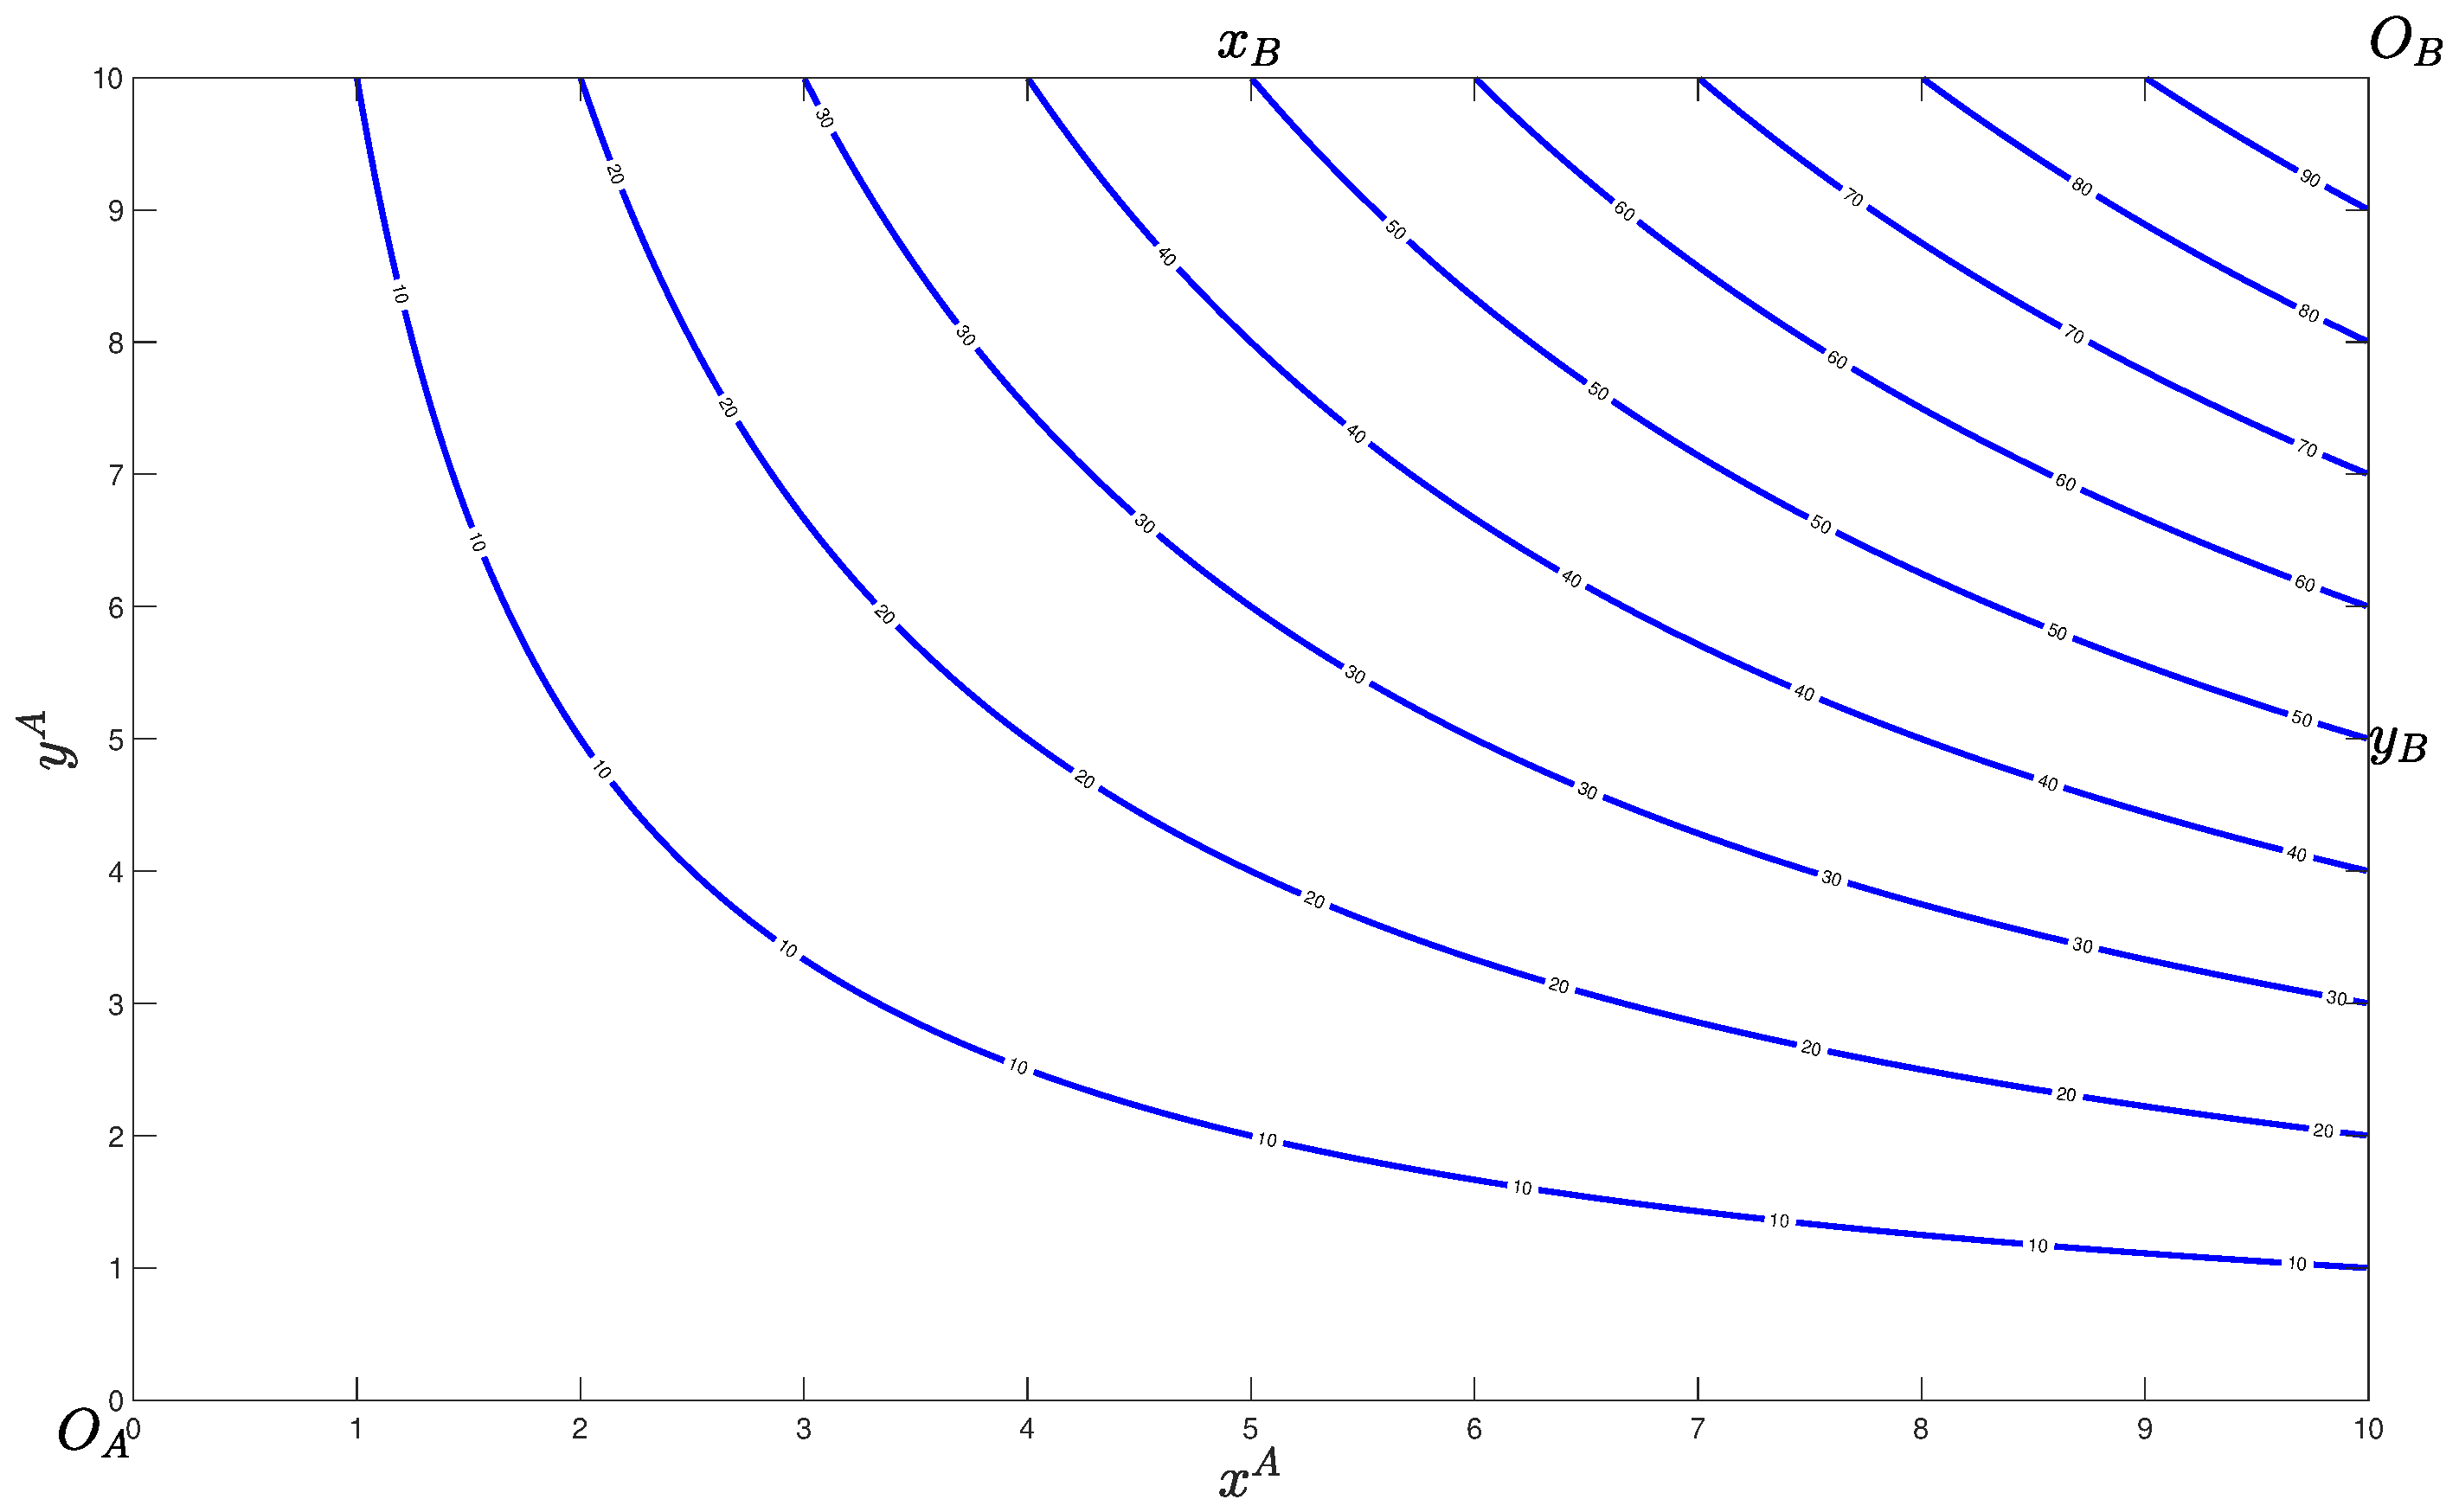
\includegraphics[width=0.7\linewidth]{Edgeworth}
\end{figure}


\end{frame}


\begin{frame}{Edgeworth Box: Indifference curves for A and B}
\begin{figure}
	\centering
	\includegraphics[width=0.7\linewidth]{Edgeworth_2}
\end{figure}


\end{frame}


\begin{frame}{Pareto Improvement}
Given an initial allocation $\left\lbrace \underline{x}, \underline{y}\right\rbrace$ we say that moving to allocation $\left\lbrace \underline{x}', \underline{y}'\right\rbrace$ generates a Pareto-improvement if and only if both $U^A(x',y')\geq U^A(x,y)$ and $U^B(x',y')\geq U^B(x,y)$, with one of the two inequalities being strict (i.e. one agent is strictly better off while the other is not worse off).
\end{frame}


\begin{frame}{Set of Pareto Improving Allocations}
\begin{figure}
	\centering
	\includegraphics[width=0.7\linewidth]{Edgeworth_2}
\end{figure}
\end{frame}

\begin{frame}{What is the contract curve?}
\begin{itemize}
	\item The contract curve identifies the set of all allocations that \textit{can be a general equilibrium of the economy} (i.e. for which there exists a price ratio that makes these point an equilibrium starting from \textit{some} initial allocation).
	\item In practice, this is the locus of points where the MRS of the two agents are equalized.
	\item Why should the MRS be equal? Well, the price ratio is the same for all the economy, and agents that satisfy the five axioms set MRS = p.
	\item  In economic logic, if the MRS are not equalized, the ``mental valuations'' of marginal goods by the two agents are not equalized so there are still beneficial exchanges that can be implemented until the two agents reach agreement on the value of marginal goods.
\end{itemize}
\end{frame}

\begin{frame}{Finding the contract curve}
In the general case, the contract curve might not have an analytical expression, but not here.
The MRS of agent A at the optimum is given by:
\[
	\frac{x^B}{y^B} = 2 p, \ \ \frac{x^A}{y^A} = p \Rightarrow \frac{x^B}{y^B} = 2\frac{x^A}{y^A}
\]
Now, remember that the contract curve requires equilibrium (that is markets clear), so $x^B = X- x^A$ and $y^B = Y - y^A$. Plug in and rearrange and you get the contract curve:
\[
	y^A = 2\dfrac{x^A}{(X + x^A)}Y.
\]
Interpretation: any allocation that satisfies this expression is an equilibrium, supported by:
\[
	\frac{x^A}{y^A} = p.
\]
However, only \textbf{one} of these equilibria will arise after exchange for given initial endowments.
\end{frame}


\begin{frame}{Which Equilibrium?}
\begin{itemize}
	\item Geometrically, the final equilibrium is given by the point on the contract curve such that the line that connects this point to the initial endowment (the price ratio) is perpendicular to the contract curve. Why?

\item The slope of the contract curve tells me the ratio between $y^A$ and $x^A$, while the price ratio gives me the opposite ratio, so the two must be reciprocals.

\item Economic reasoning: if the price ratio is such that the ratio of consumption of the two goods is not the one required by the contract curve, the two MRS are not equalized, so I am not in an equilibrium because the two agents can carry out beneficial exchanges.


\end{itemize}


\end{frame}

\begin{frame}{Which Equilibrium?}

\begin{figure}
	\centering
	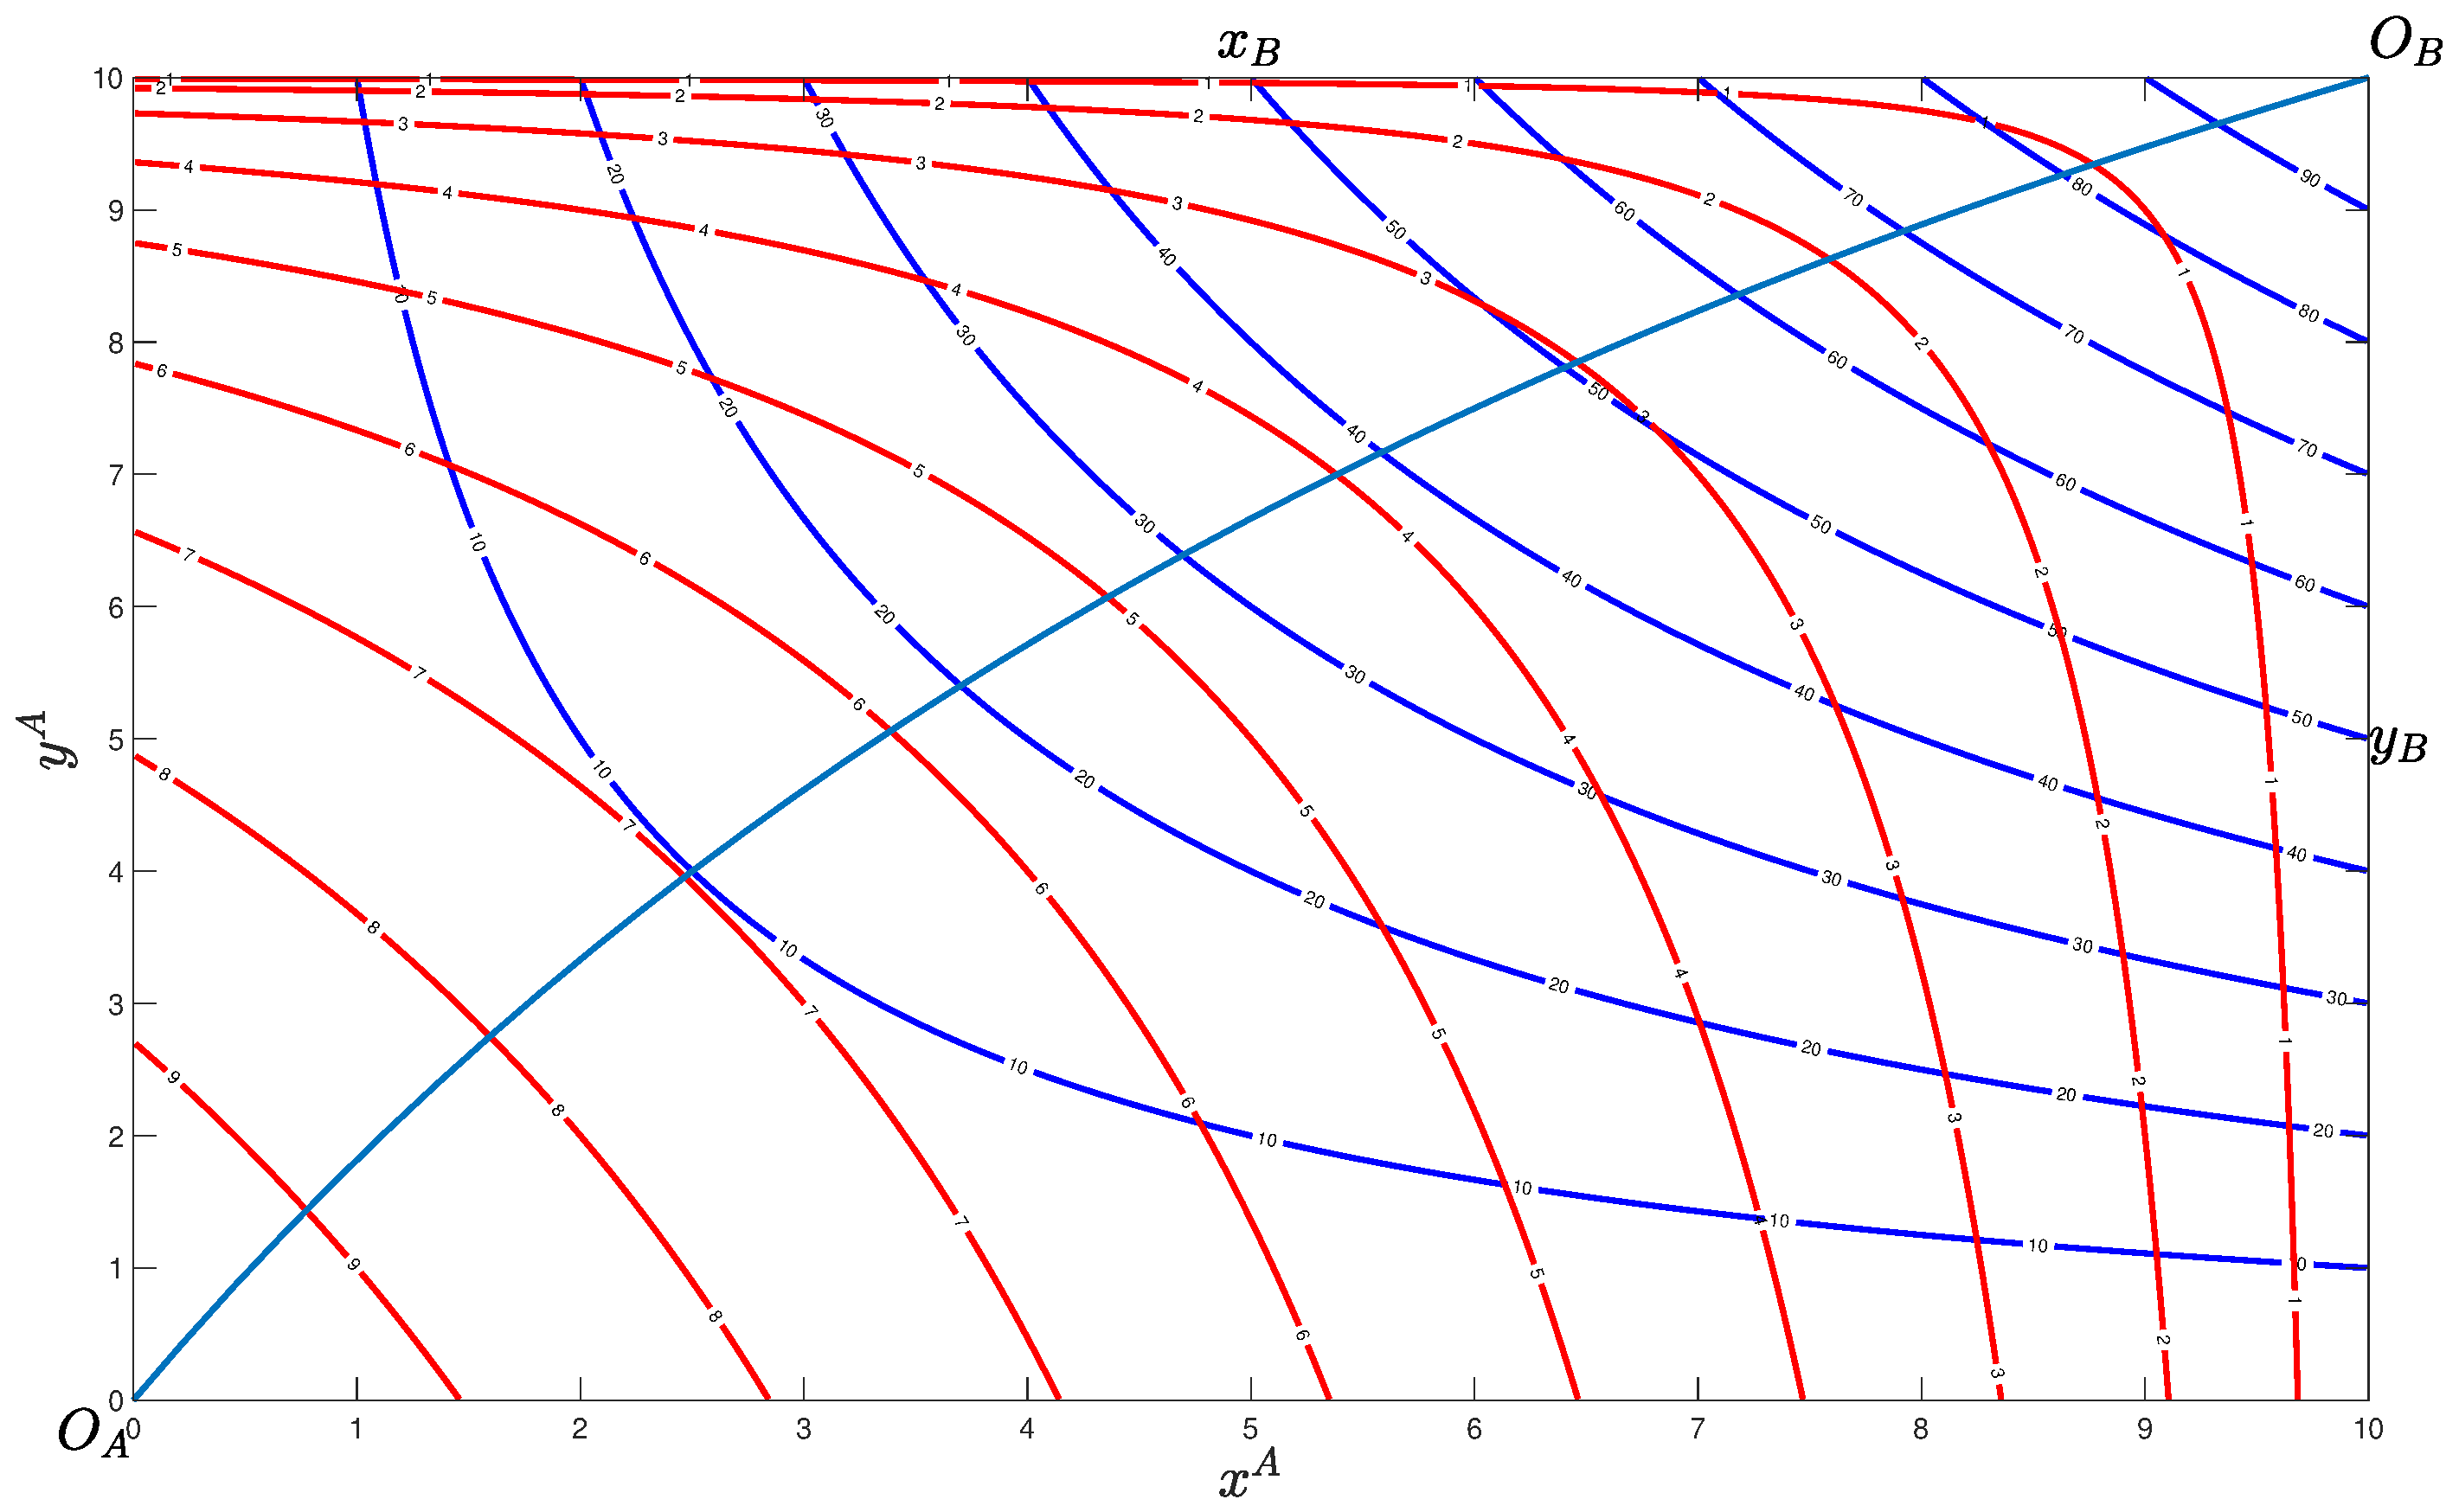
\includegraphics[width=0.7\linewidth]{Edgeworth_3}
\end{figure}

\end{frame}


\begin{frame}{General Equilibrium with Production}
A General Equilibrium is a set of \textbf{prices} $\left\lbrace p_1, p_2\right\rbrace$, and \textbf{allocations} for output, labor and consumption,  $\left\lbrace \underline{y}_1, \underline{y}_2, \underline{\ell}_1, \underline{\ell}_2, \underline{c}_1, \underline{c}_2\right\rbrace$ such that, given an endowment of labor $L$:
\begin{enumerate}
	\item Producers set output $\left\lbrace \underline{y}_1, \underline{y}_2\right\rbrace$ and choose inputs $\left\lbrace\underline{\ell}_1, \underline{\ell}_2\right\rbrace $ to  maximize profits given \textbf{prices};
	\item Consumers choose consumption $\left\lbrace \underline{c}_1, \underline{c}_2\right\rbrace$ subject to their budget constraint;
	\item  The markets for goods and labor clear.
\end{enumerate}
\end{frame}




\begin{frame}{GE with Production: Find the PPF}
\textbf{PPF}: the \textit{Production possibility frontier} is the set of all outputs that I can produce given a resource constraint. Example using only labor:
\[  y^A = \left(\ell^A\right)^\alpha, \ \ y^B = \left(\ell^B\right)^\beta.  \]
Say that total labor is 1. Then I have the constraint:
\begin{equation}\label{con}
	\ell^A + \ell^B = 1.
\end{equation}
I can obtain the PPF inverting the production functions for labor and plugging them into this constraint:
\[
	y^A = \left(\ell^A\right)^\alpha \Rightarrow \ell^A = \left(y^A\right)^\frac{1}{\alpha}, \qquad  y^B = \left(\ell^B\right)^\beta \Rightarrow \ell^B = \left(y^B\right)^\frac{1}{\beta}.
\]
Plug into \eqref{con} and rearrange:
\[
	y^B = \left(1 -\left(y^A\right)^\frac{1}{\alpha} \right)^\beta.
\]


\end{frame}

\begin{frame}{GE with Production: Graph the PPF}

\begin{figure}
	\centering
	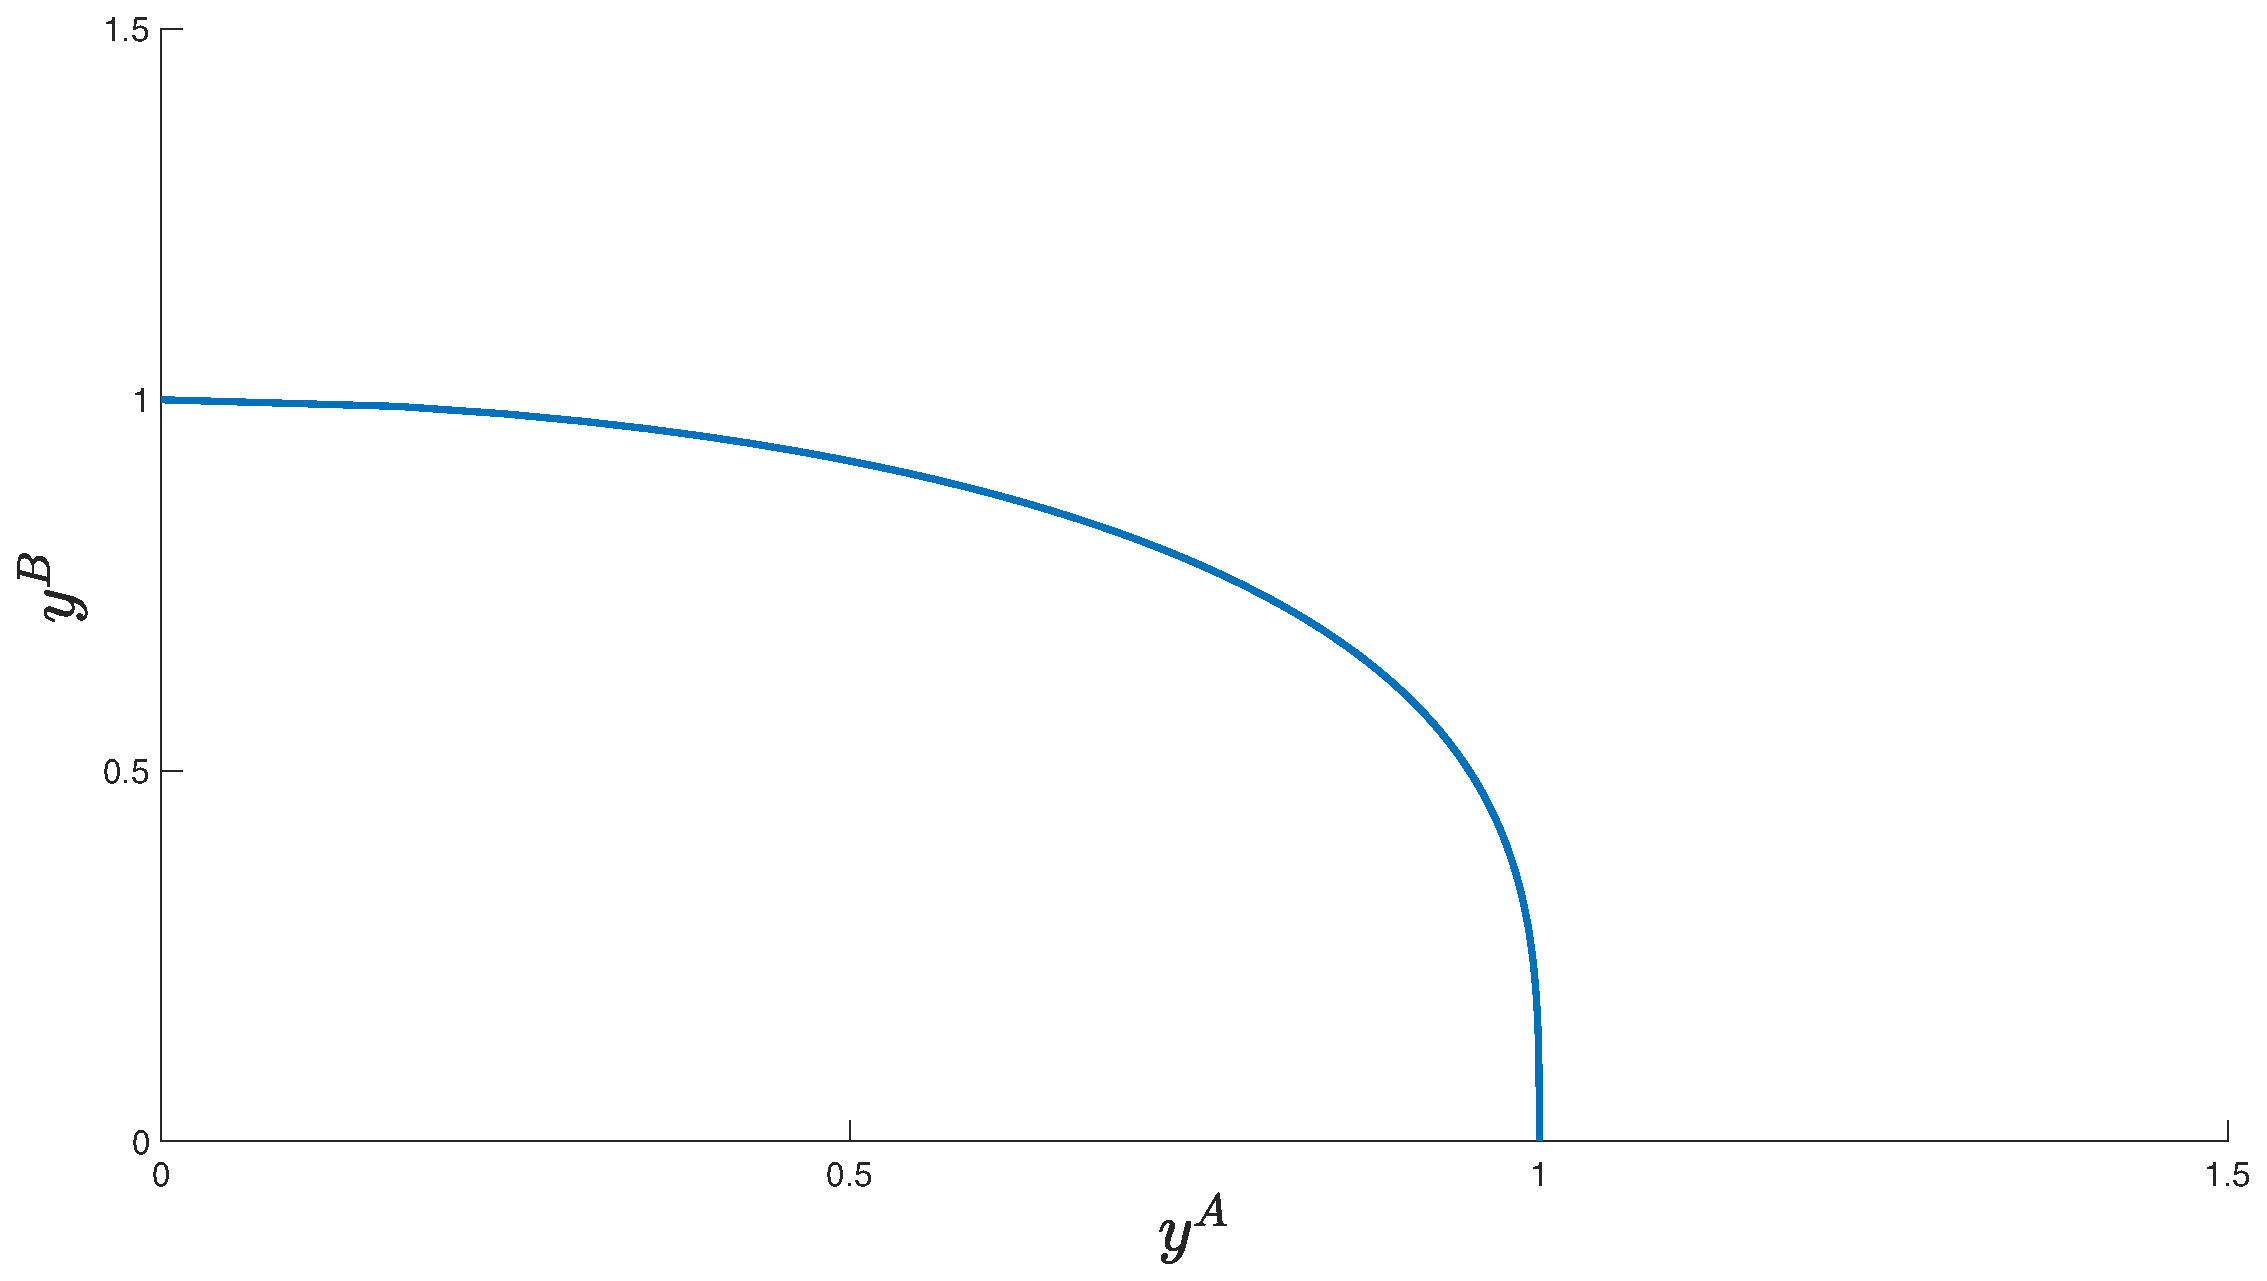
\includegraphics[width=0.7\linewidth]{PPF_only}
\end{figure}



\end{frame}

\begin{frame}{GE with Production: Equilibrium}
\begin{figure}
	\centering
	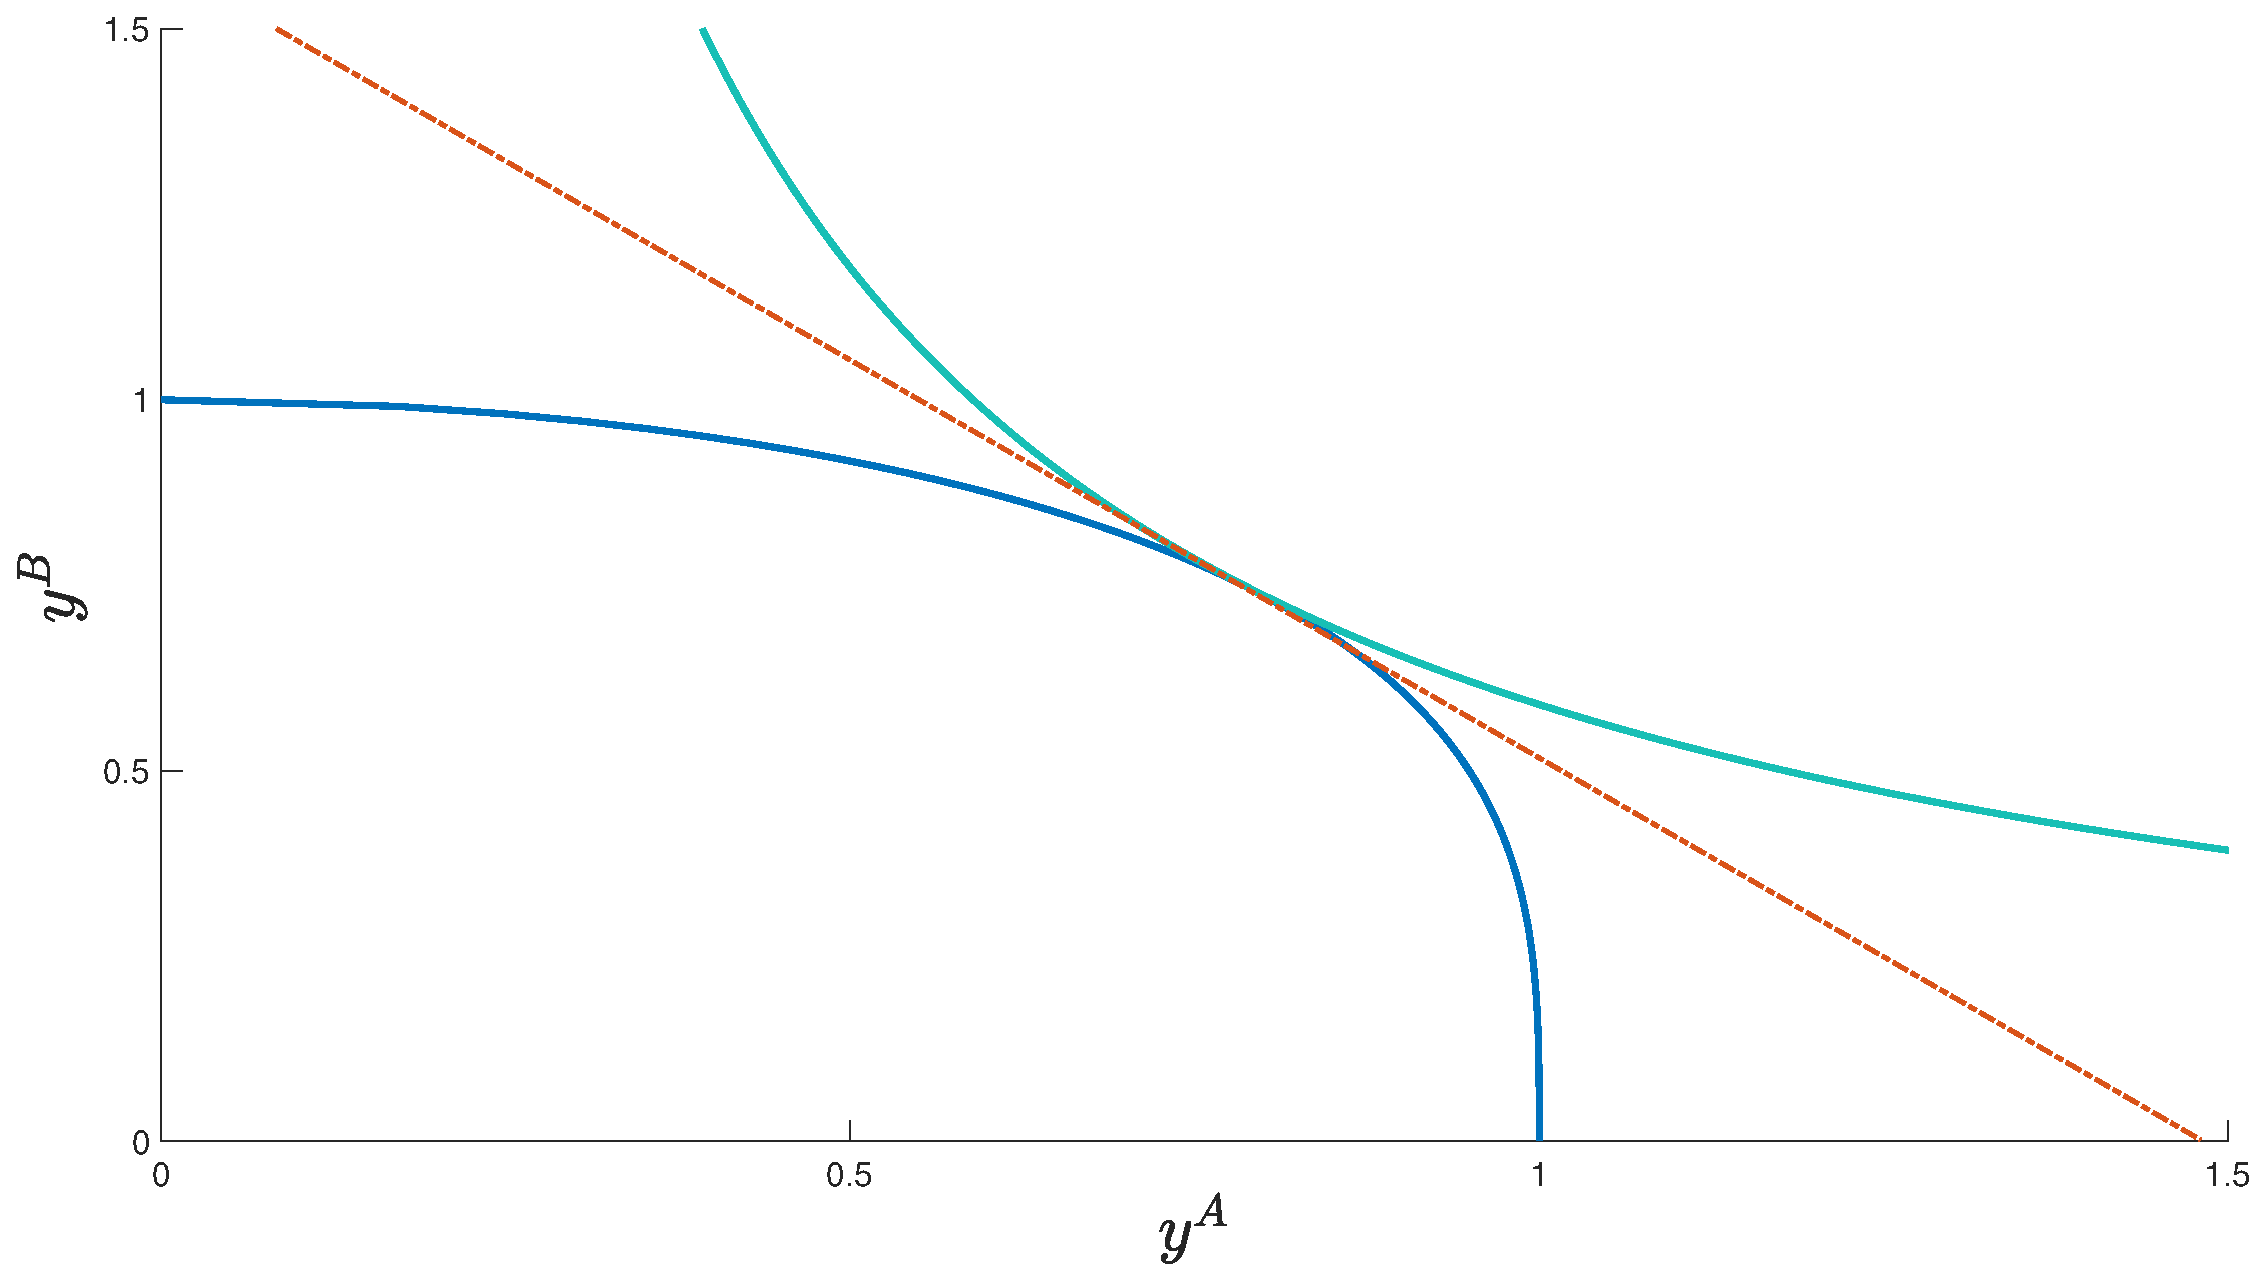
\includegraphics[width=0.7\linewidth]{PPF}
\end{figure}

\end{frame}

\begin{frame}{GE with Production: Trade}
\begin{figure}
	\centering
	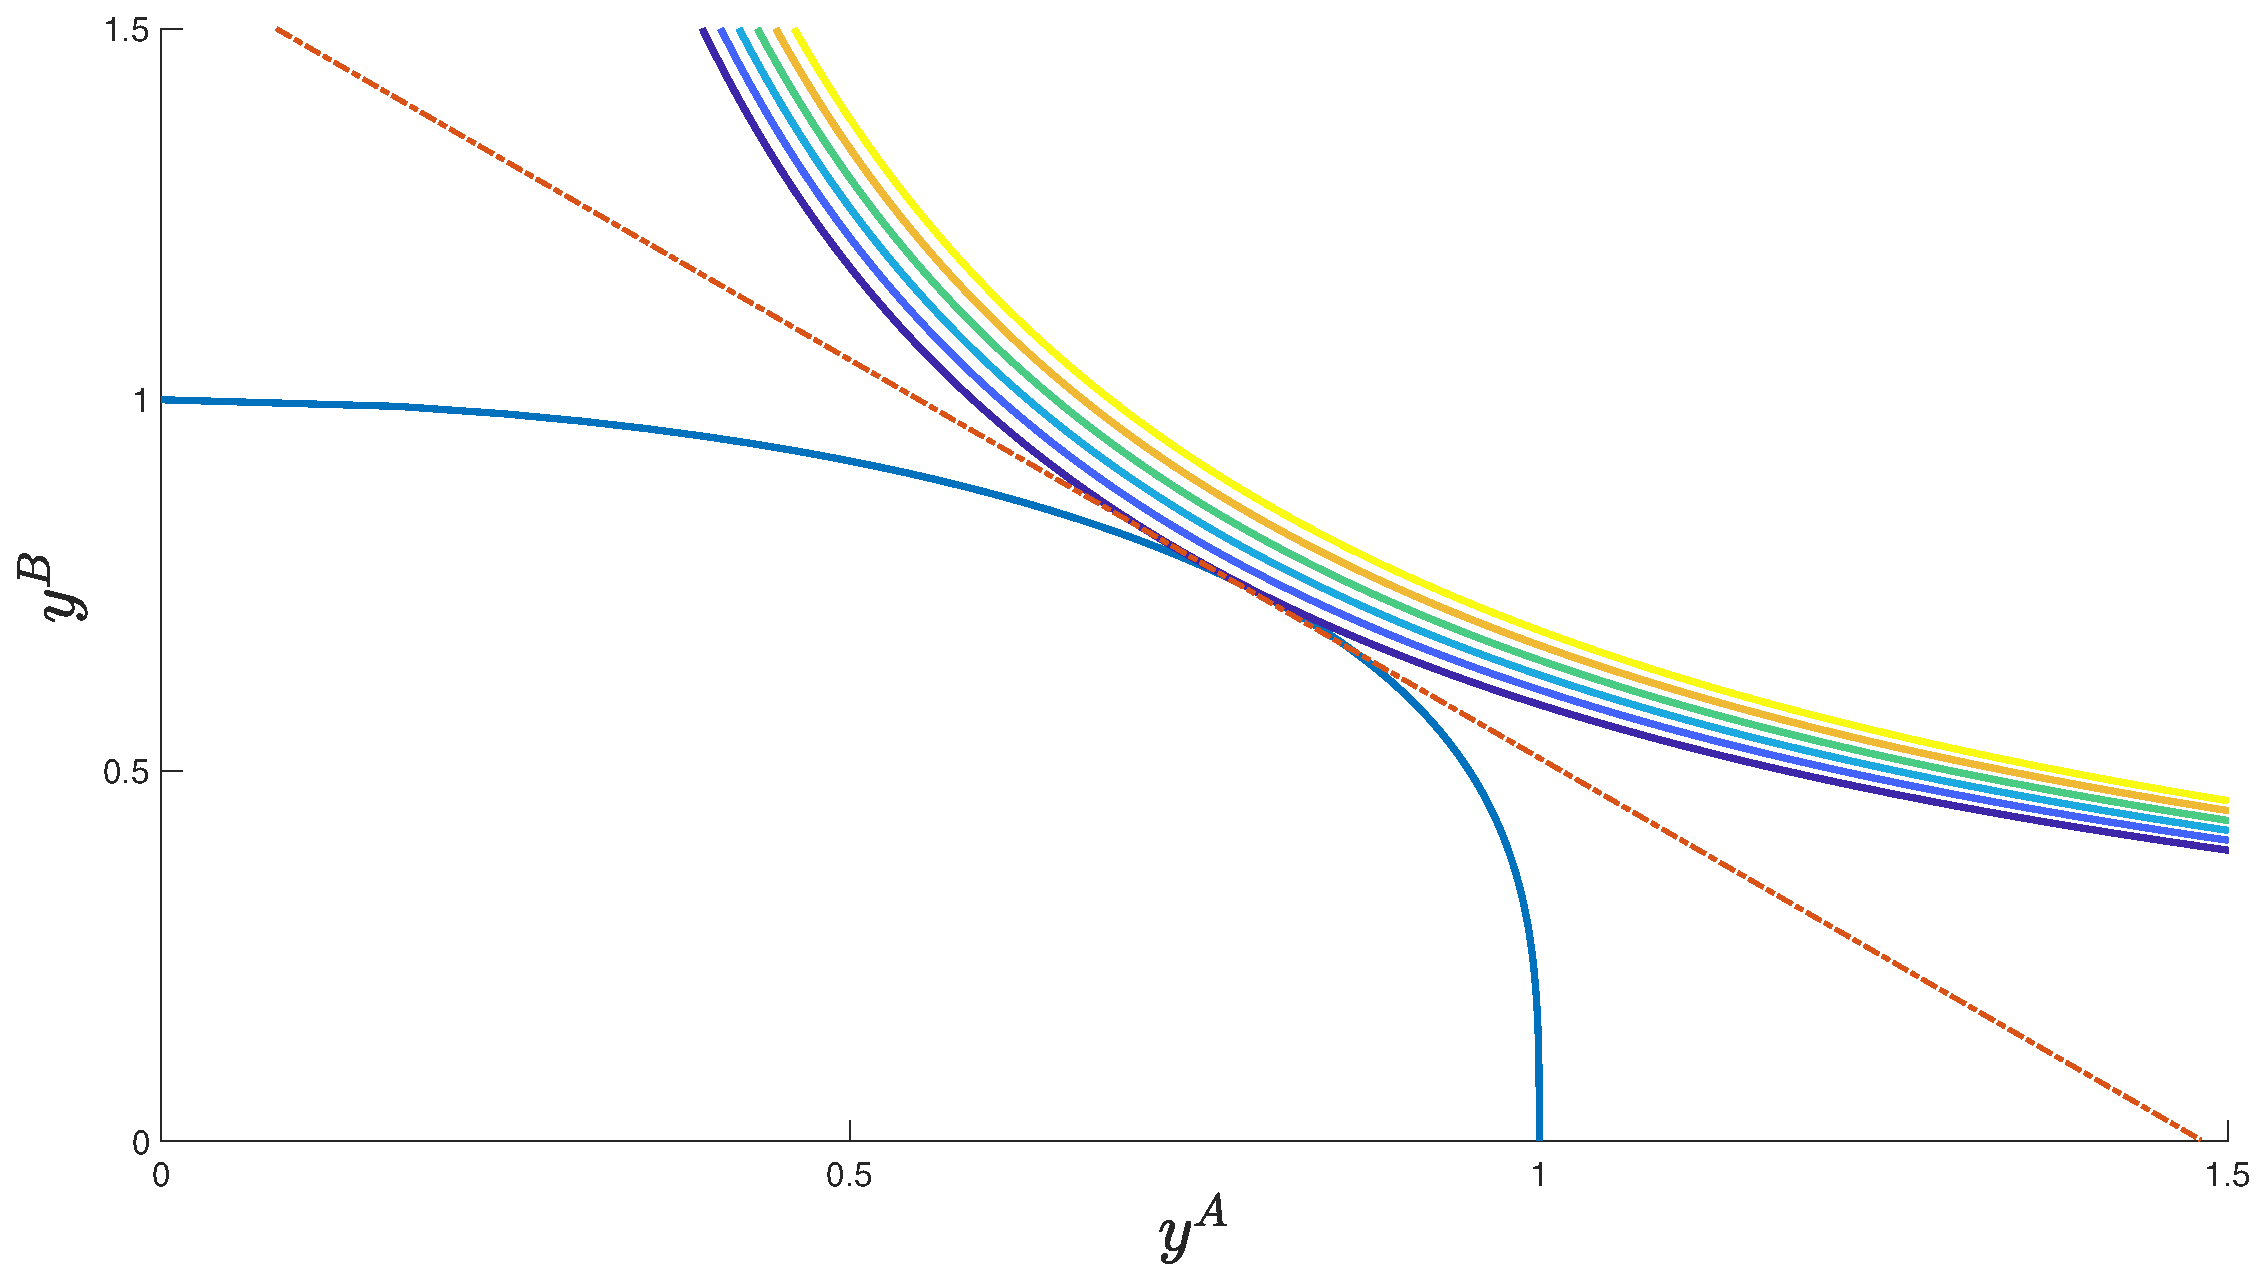
\includegraphics[width=0.7\linewidth]{PPF_2}
\end{figure}
\end{frame}